\subsection{Решение XKCD 287}
\label{XkcdILP}

\begin{figure}[H]
\centering
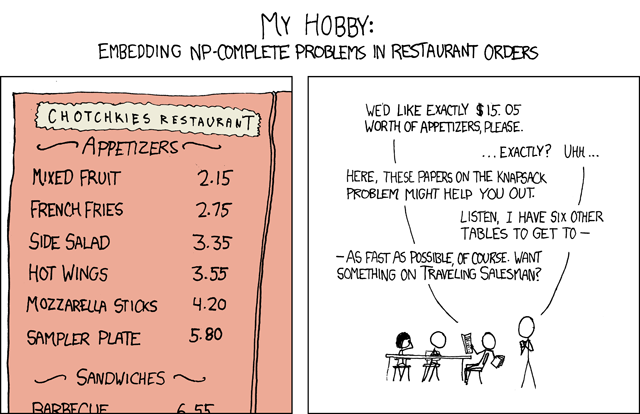
\includegraphics[scale=7]{equations/xkcd287/np_complete.png}
\caption{xkcd \#287}
\end{figure}

( \url{https://www.xkcd.com/287/} )

Вот перевод на русский, но с другими ценами:

\begin{figure}[H]
\centering

\includegraphics[scale=7]{equations/xkcd287/287_v1.png}
\caption{xkcd \#287}
\end{figure}

( \url{https://xkcd.ru/287/} )

(Но мы всё равно будем ориентироваться на цены из оригинальной англоязычной версии.)

Задача в том, чтобы решить следующее уравнение:
$2.15a + 2.75b + 3.35c + 3.55d + 4.20e + 5.80f == 15.05$,
где a..f это целочисленные.
Так что это линейное диофантово уравнение.

\lstinputlisting{equations/xkcd287/xkcd287_MK85.py}

( Исходный код: \url{https://github.com/DennisYurichev/.../xkcd287_MK85.py} )

Тут только 2 решения:

\begin{lstlisting}
{'a': 7, 'c': 0, 'b': 0, 'e': 0, 'd': 0, 'f': 0}
{'a': 1, 'c': 0, 'b': 0, 'e': 0, 'd': 2, 'f': 1}
\end{lstlisting}

Wolfram Mathematica тоже может решить это уравнение:

\begin{lstlisting}
In[]:= FindInstance[2.15 a + 2.75 b + 3.35 c + 3.55 d + 4.20 e + 5.80 f == 15.05 && 
	a >= 0 && b >= 0 && c >= 0 && d >= 0  && e >= 0 && f >= 0, 
	{a, b, c, d, e, f}, Integers, 1000]

Out[]= {{a -> 1, b -> 0, c -> 0, d -> 2, e -> 0, f -> 1},
	{a -> 7, b -> 0, c -> 0, d -> 0, e -> 0, f -> 0}}
\end{lstlisting}

1000 означает ``найти максимум 1000 решений'', но находится только 2.
См.также: \url{http://reference.wolfram.com/language/ref/FindInstance.html}.\\
\\
Другие способы решения:
\url{https://stackoverflow.com/questions/141779/solving-the-np-complete-problem-in-xkcd},
\url{http://www.explainxkcd.com/wiki/index.php/287:_NP-Complete}.

Решение используя Z3: \url{https://github.com/DennisYurichev/.../xkcd287_Z3.py} )

\subsection{XKCD 287 в формате SMT-LIB 2.x}

\lstinputlisting{equations/xkcd287/xkcd287.smt}

